% Reports (up to ~2500 words including references, notes and captions–corresponds to ~3
% printed pages in the journal) present important new research results of broad
% significance. Reports should include an abstract, an introductory paragraph, up to
% four figures or tables, and about 30 references. Materials and Methods should be
% included in supplementary materials, which should also include information needed to
% support the paper's conclusions.

% Main Text is not divided into sub-headings for Reports. 

% The manuscript should start with a brief introduction describing the paper’s
% significance. The introduction should provide sufficient background information to
% make the article intelligible to readers in other disciplines, and sufficient context
% that the significance of the experimental findings is clear. 

% \clearpage

Since early 2020, the CoViD-19 pandemic has presented an enormous challenge to humanity
on many dimensions. The development of highly effective vaccines holds the promise of
containment in the medium term. However, most countries find themselves many
months---and often years---away from reaching vaccination-induced herd
immunity.\comment[id=HM]{Cite some paper on herd immunity, maybe vaccine data} In the
meantime, it is of utmost importance to employ an effective mix of strategies for
containing the virus. The most frequent initial response was a set of non-pharmaceutical
interventions (NPIs) to reduce contacts between individuals. While this has allowed some
countries to sustain equilibria with very low infection numbers\footnote{See
\citet{Contreras2021} for a theoretical equilibrium at low case numbers which is
sustained with test-trace-and-isolate policies.}, most have seen large ups and downs in
their infection rates. Containment measures have become increasingly diverse and
included testing, more nuanced NPIs, and contact tracing. Neither these policies' effect
nor the influence of seasonal patterns or more infectious virus strains are well
understood in quantitative terms. This paper develops a model incorporating all these
factors. The framework allows to combine a wide variety of data in a timely fashion,
making it useful to predict the effects of various interventions. We apply the model to
Germany and show that rapid testing had the largest impact on the reduction in
infections by XXX\% during the A weeks between X April and Y May.\comment[id=HM]{insert
some useful numbers}. We conclude that rapid tests should play a large role...

At the core of our agent-based model are physical contacts between heterogeneous agents
(Figure~\ref{fig:broad_model_description}).\footnote{We provide a detailed comparison to
other approaches in \ref{sec:literature_review}. The model most closely related to ours
is described in \citet{Hinch2020}.} Each contact between an infectious individual and
somebody susceptible to the disease bears the risk of transmitting the virus. Contacts
occur in the household, at work, at school, or in other settings (leisure activities,
grocery shopping, medical appointments, etc.).\comment[id=HM]{Systemic relevance of
work?} Some contacts recur regularly, others occur at random. Random contacts are
typically assortative in age and geographical location. Empirical applications can take
the population structure from census data and the types and frequency of contacts from
diary data measuring contacts before the pandemic
\citep[e.g.][]{Mossong2008}.\footnote{\citet{Hoang2019} provide access to multiple data
sets on contact types and frequencies at \url{http://www.socialcontactdata.org/}
covering countries from all continents except North America and Australia.} The
dimensions are chosen so that the most common NPIs can be modeled in great detail by
reducing the number of contacts in a particular setting or the risk of transmitting the
disease for a type of contact. For example, a mandate to work from home will reduce the
number of work contacts to zero for a fraction of the working population. Schools and
daycare can be closed entirely, operate at reduced capacity including an alternating
schedule, or implement mitigation measures like masking requirements or air filters
\citep{Lessler2021}. Curfews may reduce the number of contacts in non-work/non-school
settings. In any setting, measures like masking requirements would reduce the
probability of infection associated with a contact.

\begin{figure}[!tp]
    \centering

    \begin{subfigure}[b]{0.425\textwidth}
        \centering
        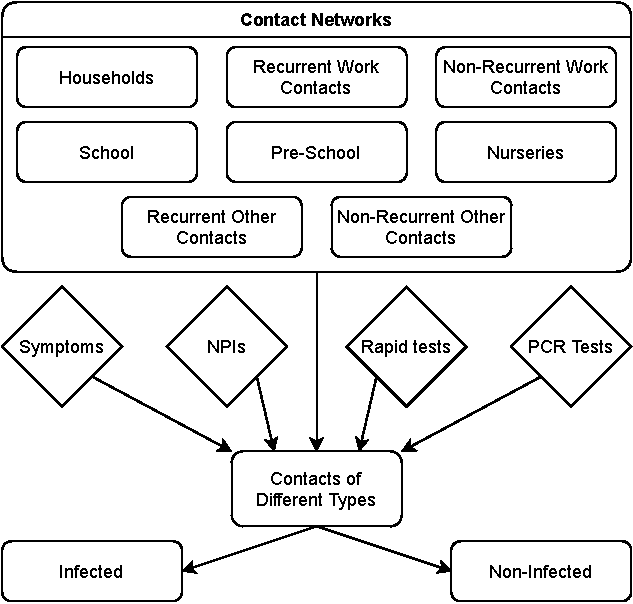
\includegraphics[width=\textwidth]{../figures/model-graph-top-left}
        \caption{{\small Model description}}
        \label{fig:broad_model_description}
    \end{subfigure}
    \hfill
    \begin{subfigure}[b]{0.425\textwidth}
        \centering
        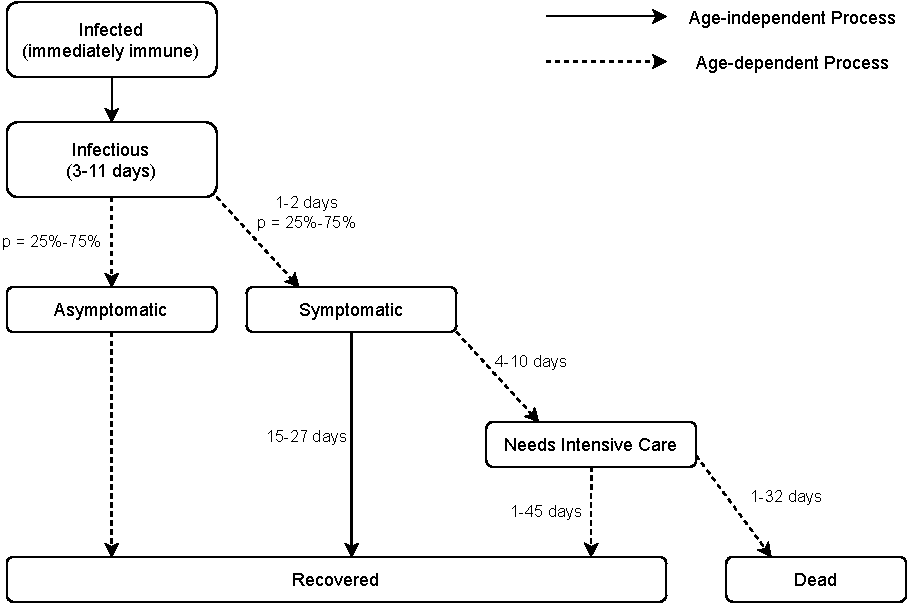
\includegraphics[width=\textwidth]{../figures/model-graph-top-right}
        \caption{Disease progression}
        \label{fig:disease_progression}
    \end{subfigure}
    \vskip3ex
    \begin{subfigure}[b]{0.425\textwidth}
        \centering

        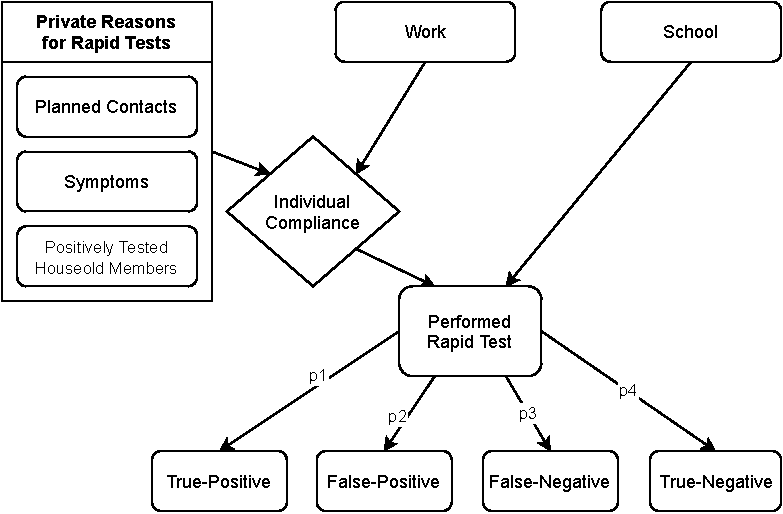
\includegraphics[width=\textwidth]{../figures/model-graph-bottom-left}
        \caption{{\small PCR and antigen tests}}
        \label{fig:pcr_antigen_tests}
    \end{subfigure}
    \hfill
    \begin{subfigure}[b]{0.425\textwidth}
        \centering

        Model for detected/undetected cases

        % 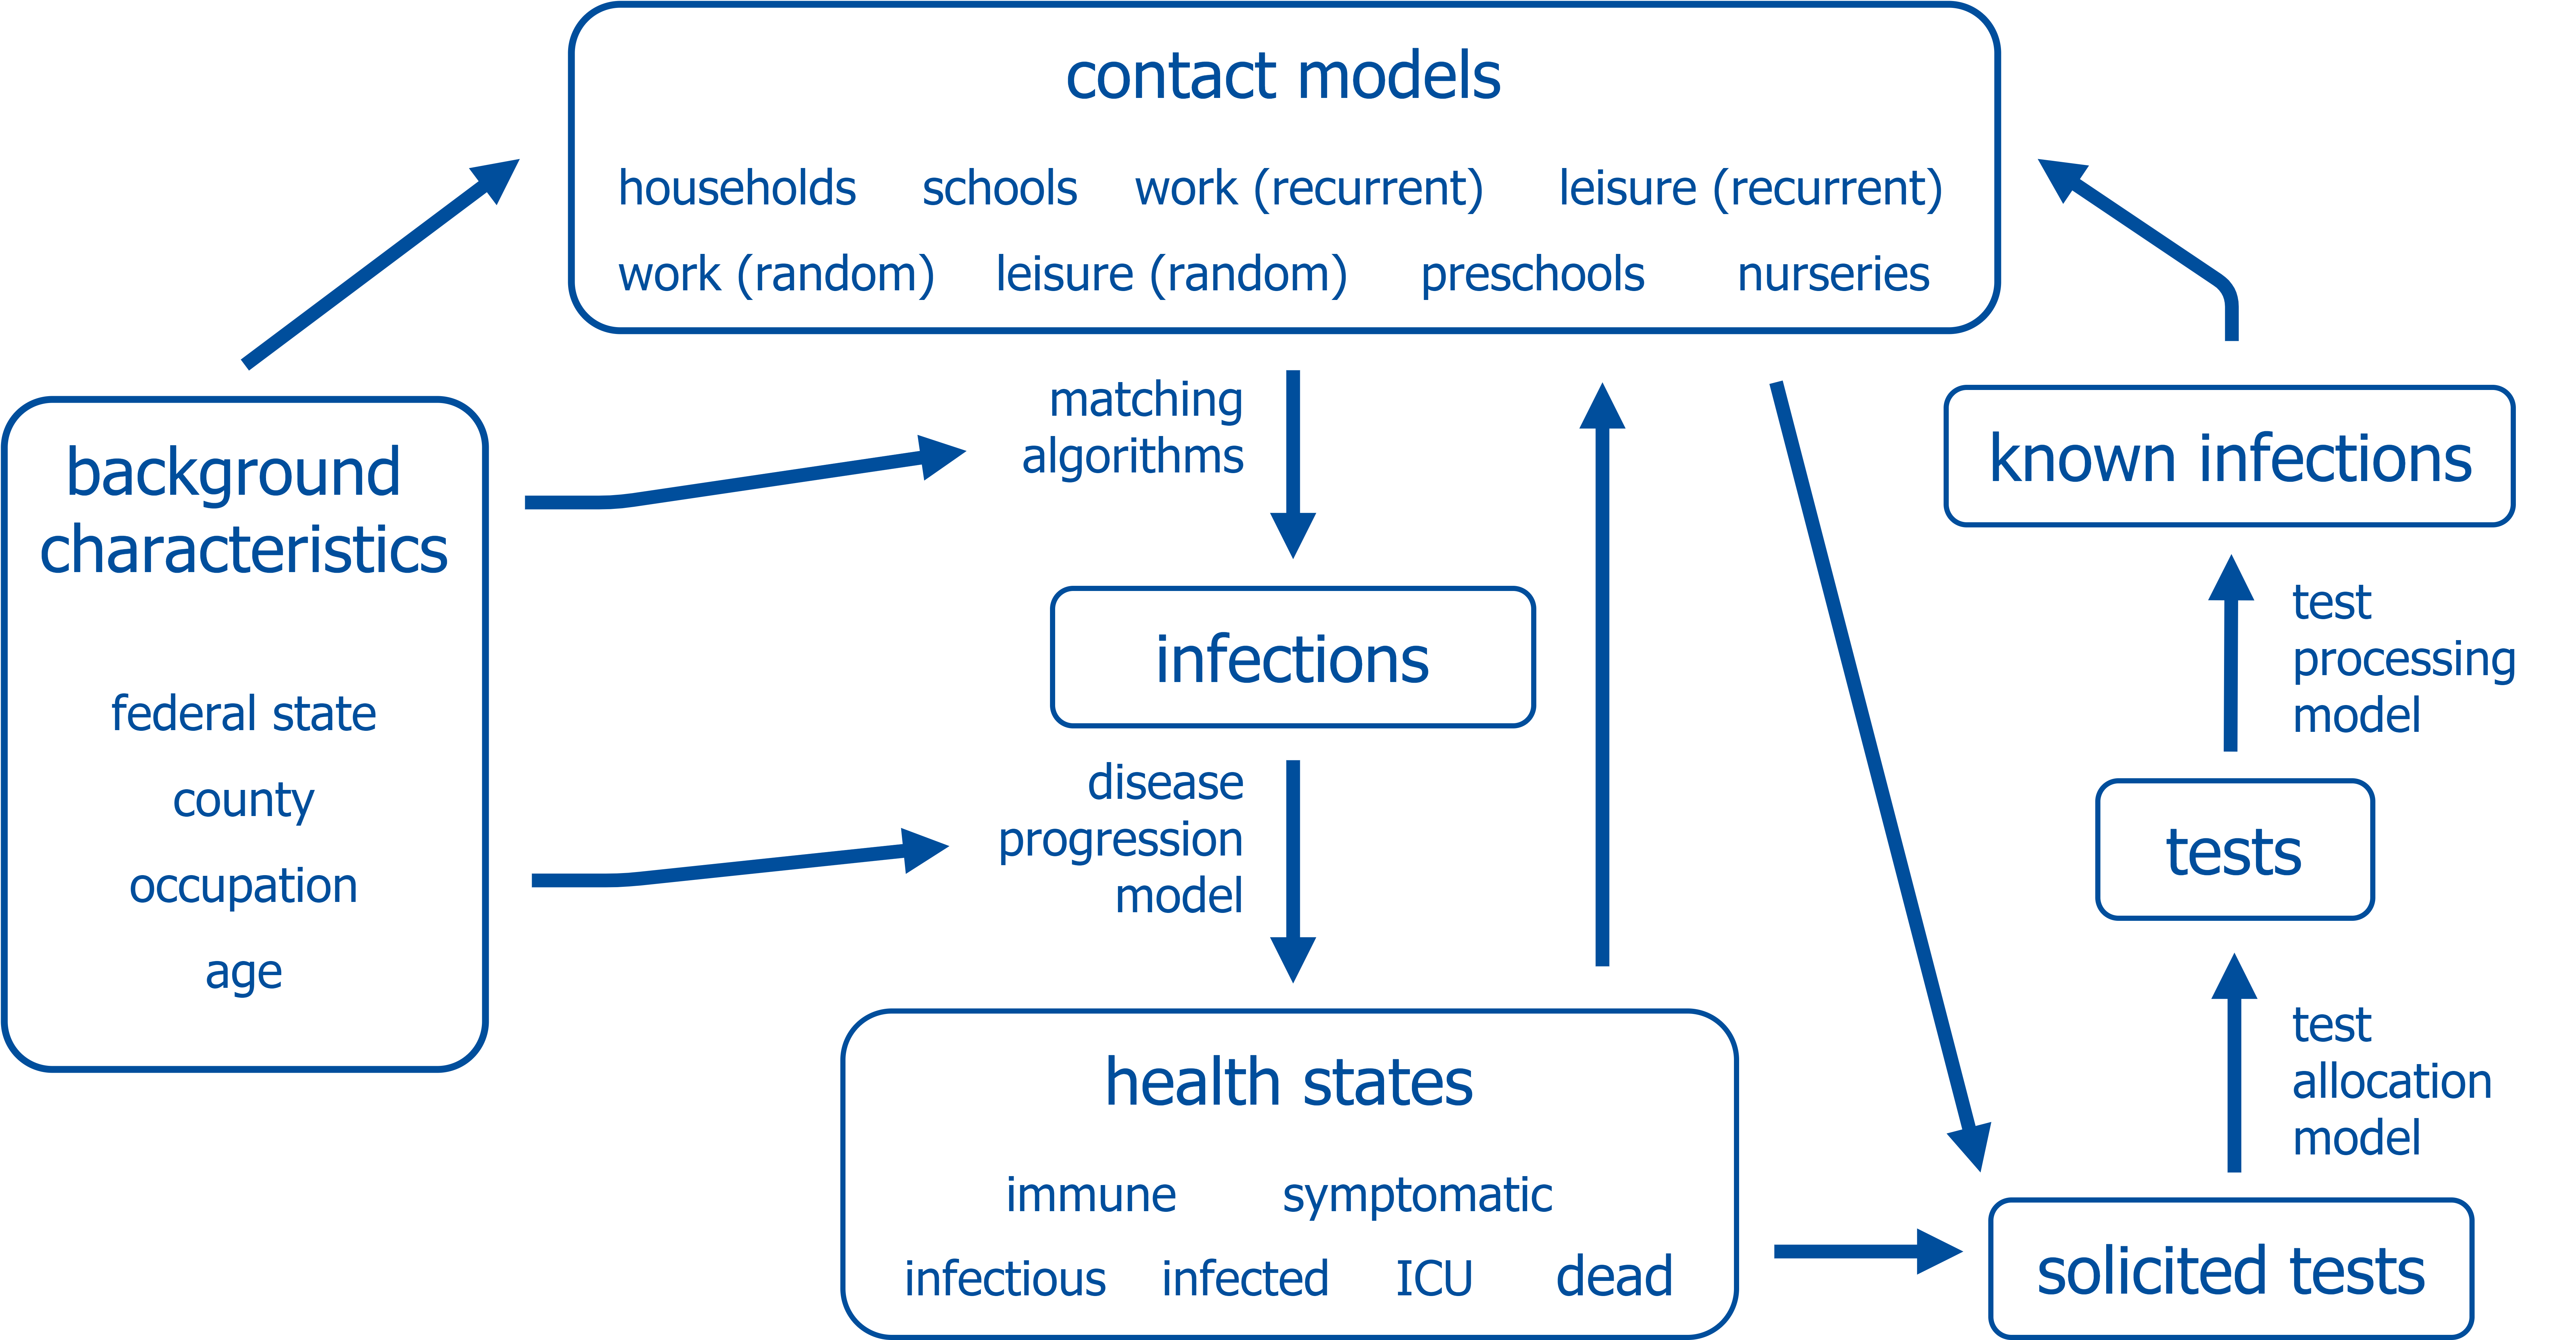
\includegraphics[width=\textwidth]{../figures/model_detailed.png}
        \caption{{\small Model for translating simulated number to officially recorded
        cases}}
        \label{fig:model_for_official_cases}
    \end{subfigure}

    \caption{Model description}
    \label{fig:model-description}

    \floatfoot{\noindent Note: ...}
\end{figure}

EQUATIONS FOR THE FOURTH PICTURE (find names!):

The probabilities for Figure~\subref{fig:model_for_official_cases} are the following:

\begin{align*}
    x &= \frac{n\_newly\_infected \times share\_known\_cases \times P(PCR | S)}{n\_symptomatic\_and\_untested} \\
    y &= \frac{n\_newly\_infected \times share\_known\_cases \times P(PCR | S)}{n\_asymptoptomatic\_and\_infected\_and\_untested} \\
    z &= \frac{P(PCR | RT)}{survey}
\end{align*}

where untested means that individuals are not waiting on the result of a previously
administered rapid test.

Susceptibility to contracting the SARS-CoV-2 virus is dependent on age; so is the
progression of a possible infection. We differentiate between an initial period of
infection without being infectious or showing symptoms, being infectious (presymptomatic
or asymptomatic), showing symptoms, requiring intensive care, and recovery or death. The
probabilities of transitioning between these states depend on age; their duration is
random within intervals calibrated to medical literature (for a detailed description see
Section~\ref{sec:medical_params}). Conditional on the type of contact, infectiousness
independent of ages \citep{Jones2021}.

The model includes several other features, which are crucial to describe the evolution of
the pandemic in 2020-2021. New virus strains with different profiles regarding
infectiousness \replaced[id=K]{and disease progress}{}\comment[id=K]{sid only supports
differing infectiousness between variants at the moment} can be introduced. With a
probability of 75\% \citep{Hunter2021}, vaccinated agents become immune and they do not
transmit the virus \citep{Petter2021, LevineTiefenbrun2021, Pritchard2021}.\footnote{75\%
is lower than what is usually reported for after the second dose. We choose it because in
our model does not include booster shots and does not allow for vaccinated individuals to
become infected and transmit the disease which is the case for Covid-19
\citep{Petter2021, LevineTiefenbrun2021, Pritchard2021}.}% the sources only report reduced viral shedding and reduced risk of infection.
% Lauterbach calculated that taking the risk of infection * reduced infectiousness given
% infection based on theses studies suggest that given exposure the risk that fully
% vaccinated individuals pose is <10% of an unvaccinated person.
While vaccines are rolled out, priority depends on age and occupation. Agents may
demand two types of tests as described in Figure~\ref{fig:pcr_antigen_tests}. First,
polymerase chain reaction (PCR) tests directly reveal whether an individual is infected
or not. PCR tests require some time to be processed and there are always aggregate
capacity constraints. Second, rapid antigen tests yield immediate results. Specificity
and sensitivity of these tests is set according to data by \cite{Bruemmer2021,
Smith2021} . The sensitivity of the rapid antigen tests depends on the timing of the
test relative to the start of infectiousness.\comment[id=HM]{subsequent PCR tests,
quarantine, work/school}. Demand for rapid tests will depend on policy, e.g., prices,
testing requirements before work, attending school, or visiting restaurants and shops.

Modelling a population of agents according to actual demographic characteristics means
that we can use a wide array of data to identify and estimate the model's many
parameters.\footnote{See section S.X of the supplementary materials for an
overview.}\comment[id=HM]{Need to make a list including symbols, maybe you can fetch the
parameters from the model and then we brainstorm re notation?} Mobility data is used to
model the reductions in work contacts. School and daycare policies are incorporated
directly from official directives. Infection rates by age and geographical region are
estimated to match to officially recorded numbers; so is the prevalence of virus strains.
In order to translate simulated cases in our model to officially recorded cases, we use
the model depicted in Figure~\ref{fig:model_for_official_cases}.\comment[id=HM]{Add a
sentence.} A further advantage is that the simulated data have a structure that resembles
datasets used for regression models, which allows additional plausibility checks by
re-running the same models on the model-generated data.\comment[id=HM]{Only keep if we
actually do something like that.}

Model that makes the most of many available data sources to gauge the relative effects
in this transition period -- see joint distribution of infections with age, geography.
But contacts with age, geography, occupations.

We apply this model to Germany. In March and April 2020, the country broke the first
wave of the pandemic fairly quickly. Between mid-May and mid-September, daily new
infections were below 20 per Million and day.\comment[id=HM]{Cite our world in data} We
model the period mid-September 2020 to the end of May 2020. We pick the starting date
for two reasons. First, we do not include the first wave because the environment was
very different (e.g., aggregate PCR test capacity was much lower and we would require a
very different model for calculating the share of known cases) and some data was not
recorded yet.\comment[id=HM]{True?}\comment[id=K]{We would definitely need to model
national and international travel which you mention below. Regarding data I think
everything would be available. The low numbers during summer in our sample size might
also be a problem because Covid might go extinct in our model when case numbers are so
low.}. Second, a large fraction cases during summer of 2020 were traced to international
travel \citep{KochInstitut2021}, but the precise number is difficult to model.

Figure~\ref{fig:pandemic_drivers_model_fit} describes the evolution of the pandemic and
of its drivers. The black line in Figure~\ref{fig:aggregated_fit} shows officially
recorded cases; the \replaced[id=HM]{color}{blue?} line in
Figure~\ref{fig:stringency_index} the Oxford Response Stringency Index \citep{Hale2020},
which tracks the tightness of non-pharmaceutical interventions. We transform the index
so that lower values represent higher levels of restrictions. A value of zero means all
measures incorporated in the index are turned on. The value 1 represents the situation
of mid-September, where half of all restrictions incorporated in the index are
active.\comment[id=HM]{Need to find version of index with a couple of measures, probably
need the API access...}. In the six weeks between mid September and late October, cases
increased by a factor of XX.\comment[id=K]{In the next iteration all empirical data is
in the figures/results/tables/empirical\_analogues.csv}
% the week of Sep 13 had an incidence of 12.4, the week of Oct 18 had 51.
Restrictions were somewhat tightened in mid-October and again in early November. New
infections remained constant throughout November, before rising again in December.

\begin{figure}[!tp]
    \centering

    \begin{subfigure}[b]{0.475\textwidth}
        \centering
        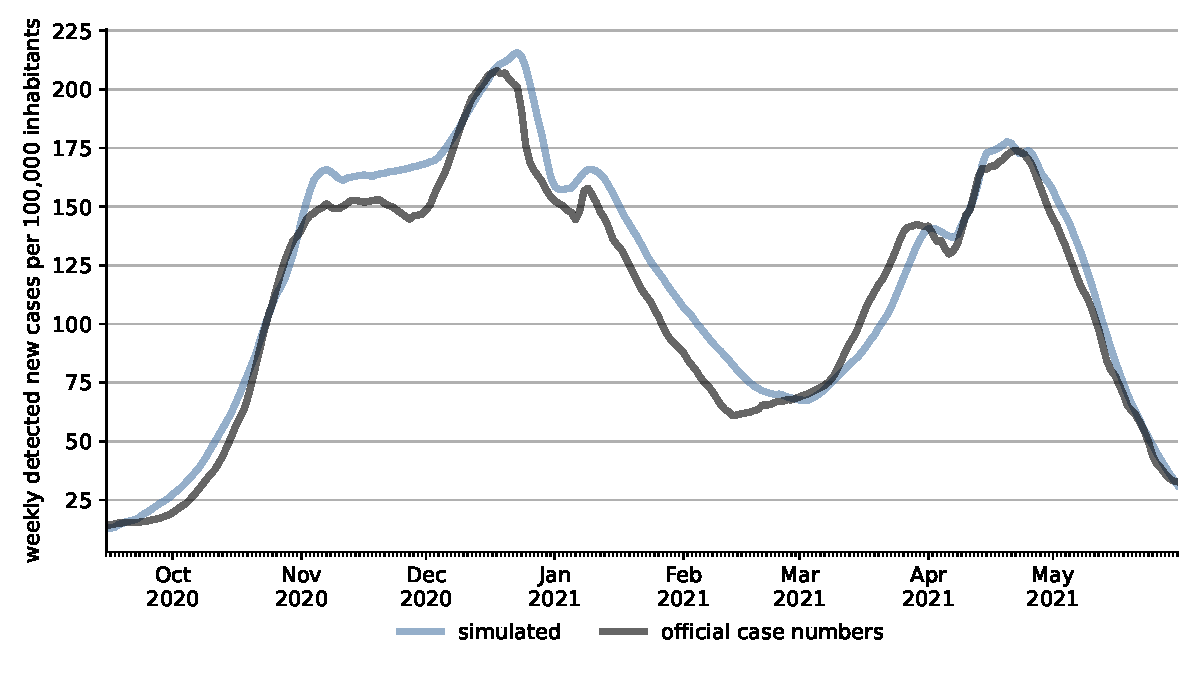
\includegraphics[width=\textwidth]{../figures/results/figures/scenario_comparisons/combined_fit/full_new_known_case}
        \caption{{\small Recorded cases: Empirical and simulated}}
        \label{fig:aggregated_fit}
    \end{subfigure}
    \hfill
    \begin{subfigure}[b]{0.475\textwidth}
        \centering
        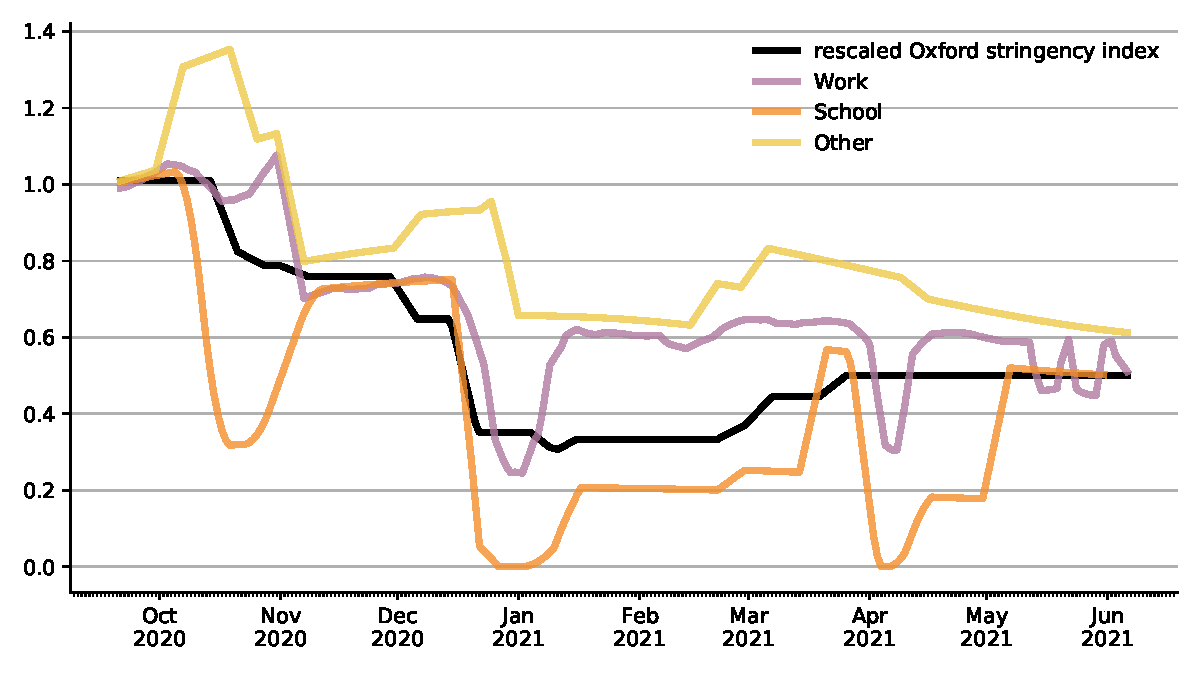
\includegraphics[width=\textwidth]{../figures/results/figures/data/stringency2_with_seasonality}

        \caption{{\small Stringency of NPIs and changes in infectious contacts by type}}
        \label{fig:stringency_index}
    \end{subfigure}

    \vskip3ex

    \begin{subfigure}[b]{0.475\textwidth}
        \centering

        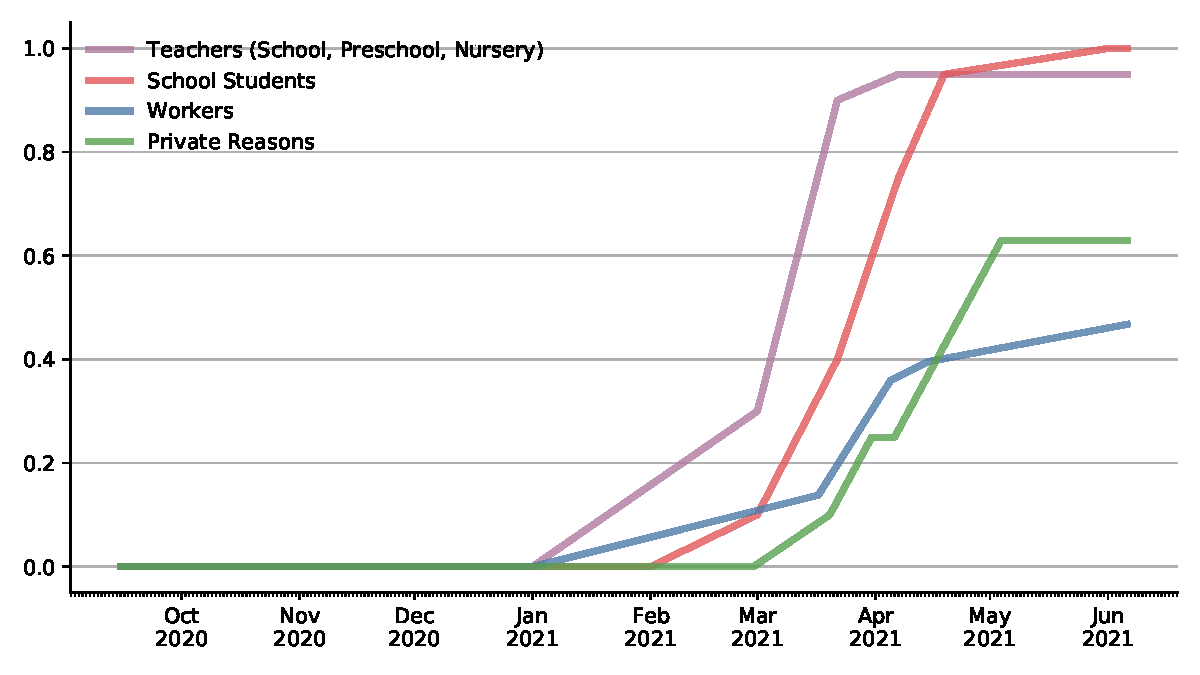
\includegraphics[width=\textwidth]{../figures/results/figures/data/testing/rapid_test_demand_shares}

        \caption{{\small Tests and vaccinations}}
        \label{fig:antigen_tests_vaccinations}
    \end{subfigure}
    \hfill
    \begin{subfigure}[b]{0.475\textwidth}
        \centering

        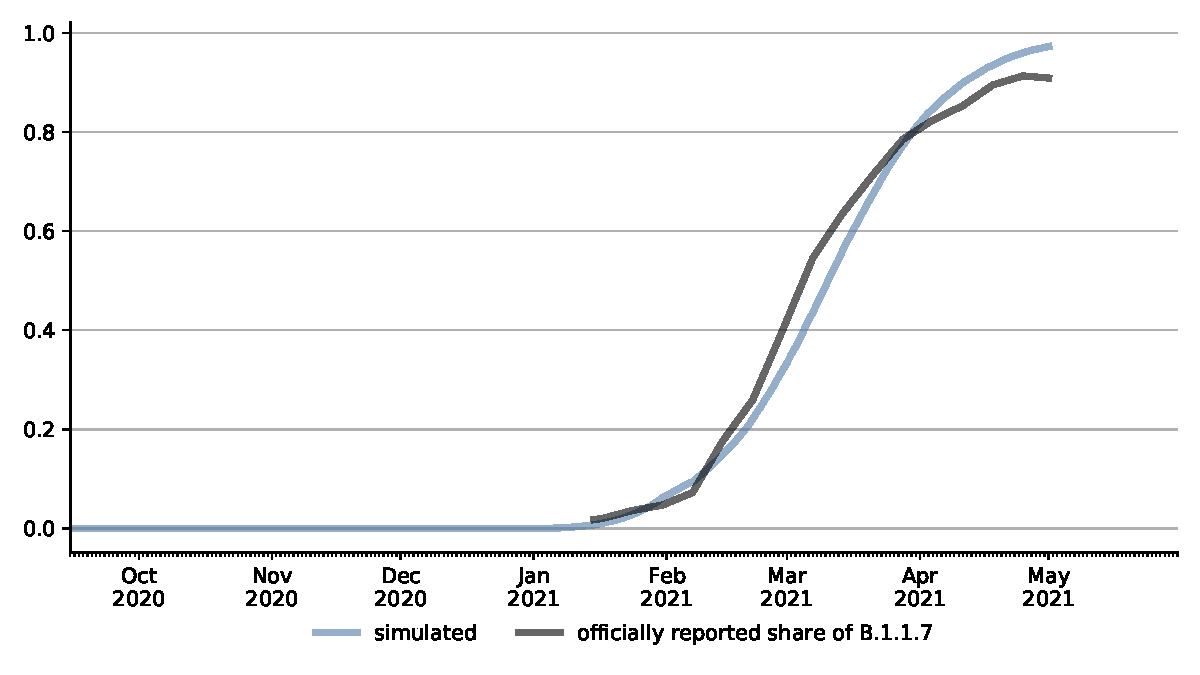
\includegraphics[width=\textwidth]{../figures/results/figures/scenario_comparisons/combined_fit/full_share_b117}

        \caption{Fraction of B.1.1.7 strain among measured infections}
        \label{fig:share_b117}
    \end{subfigure}

    \caption{Evolution of the pandemic, its drivers, and model fit, September 2020 to May 2021}
    \label{fig:pandemic_drivers_model_fit}

    \floatfoot{\noindent Note: All aggregates; See S.XXX for statistics by age group and
        by geographical region. Also more disaggregated data.

        Sources: ...}

\end{figure}

Quickly rising rates in December prompted the most stringent lockdown to this date.
Schools and daycare centers were closed again, so were customer-facing businesses except
for grocery and drug stores. Shortly afterwards, more factors become relevant. Just
after Christmas, the first people were vaccinated with a focus on older age groups and
medical personnel (Figure~\ref{fig:antigen_tests_vaccinations}. By the end of May, just
over 40\% had received at least one dose of a vaccine. Starting in January, rapid tests
\dots These had to be administered by medical doctors or in pharmacies. At-home tests
approved by authorities were ... in March.\comment[id=HM]{update precise
timeline}\comment[id=K]{From a docstring:Bürgertests started in mid March but demand was
very low initially (\url{https://bit.ly/3ehmGcj}). First tests to self-administer became
available starting March 6. However, supply was very limited in the beginning
(\url{https://bit.ly/3xJCIn8}). The first tests were licensed on Feb 24:
\url{https://www.bundesregierung.de/breg-de/themen/coronavirus/zulassung-schnell-test-1861354}}
From the peak of the second wave just before Christmas until the trough in mid-February,
newly detected cases decreased by almost three quarters. The third wave in the spring of
2021 is associated with a rise in the share of the B.1.1.7 variant among all infections,
depicted in Figure~\ref{fig:share_b117}, reaching more than 80\% in
April\comment[id=HM]{Do we have the table somewhere?}\comment[id=K]{Will be part of the
empirical analogues table}. In early March, some NPIs were being relaxed; e.g.,
hairdressers and home improvement stores were allowed to open again to the public. In
some cases, customers were only allowed to enter with a recent negative rapid test
result.

These developments are characteristic of many countries: The initial focus on NPIs to
slow the spread of the disease has been accompanied by vaccines and a growing acceptance
and use of rapid tests. At broadly similar points in time, novel strains of the virus
have started to pose additional challenges. The blue line in
Figure~\ref{fig:aggregated_fit} shows that our model tracks the simulated infections
extremely well. This is also true for infections by age and geographical region, which
are shown in the supplementary materials (figures~\ref{fig:age_group_fit,
fig:state_fit}. We can disentangle various mechanisms due to the distinct temporal
variation in the drivers of the pandemic. Next to the stringency index, the three lines
in Figure~\ref{fig:stringency_index} summarize how contact reductions, increased hygiene
regulations, and seasonality evolved since early September for each of the three broad
contact networks. For example, a value of 0.75 for the work multiplier means that if the
environment was the same as in September (levels of infection rates, no rapid tests or
vaccinations, only the wildtype virus present), infections at the workplace would be
reduced by 25\%. This reduction is the product of the effect of contact reductions,
increased hygiene regulations, and seasonality. Along with the levels of infections,
these measures completely determine the spread of SARS-CoV-2 in
2020.\comment[id=HM]{True?} See Appendix~\comment[id=HM]{Reference} \comment[id=K]{We
have not done the decomposition for 2020 yet. Is on my todo list} for their individual
contributions. Two things are particularly interesting. First, all lines broadly follow
the stringency index and they would do so even more if we left out seasonality. Second,
the most stringent regulations are associated with the period of strong decreases in new
infection between late December 2020 and mid-February 2021. The measures were not
enough, however, to stop the B.1.1.7 variant from spreading in the subsequent period.
The steep drop in recorded cases during May 2021 is associated with rapid tests to
X-Y~percent of the population, a vaccination rate that rose from 25\% to 4X\%, and
mostly seasonality impacting a fall in the relative infectiousness of contacts outside
of work and school\comment[id=HM]{check with corrected graph}.

Figure~\ref{fig:2021_scenarios_broad} consider the relative effects of rapid tests,
vaccinations, and of seasonality during 2021, assuming NPIs to have evolved the same way
as in the baseline scenario. Figure~\ref{fig:2021_scenarios_recorded} shows the model
fit (the bold blue line\comment[id=HM]{Make sure this is the case}, same as in
Figure~\ref{fig:aggregated_fit}), a scenario without any of the three factors (x line),
and three scenarios turning these factors off one by one.
Figure~\ref{fig:2021_scenarios_newly_infected} does the same for total infections in the
model. Figure~\ref{fig:2021_scenarios_decomposition} employs Shapley values to decompose
the difference in total infections between the scenario without any of the three factors
and our main specification.

\begin{figure}[!tp]
    \centering

    \begin{subfigure}[b]{0.475\textwidth}
        \centering
        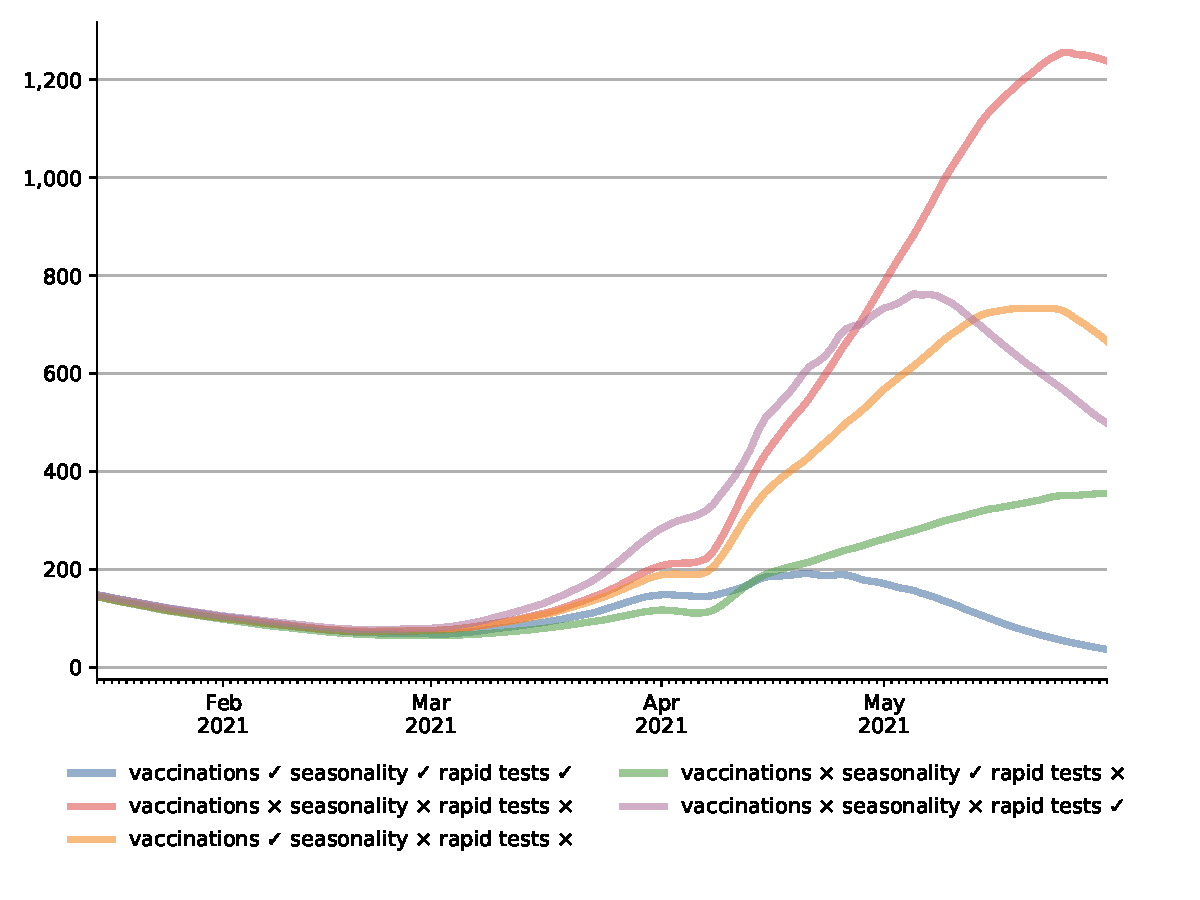
\includegraphics[width=\textwidth]{../figures/results/figures/scenario_comparisons/effect_of_channels_on_pessimistic_scenario/full_new_known_case}
        \caption{{\small Recorded cases: 2021 scenarios}}
        \label{fig:2021_scenarios_recorded}
    \end{subfigure}
    \hfill
    \begin{subfigure}[b]{0.475\textwidth}
        \centering
        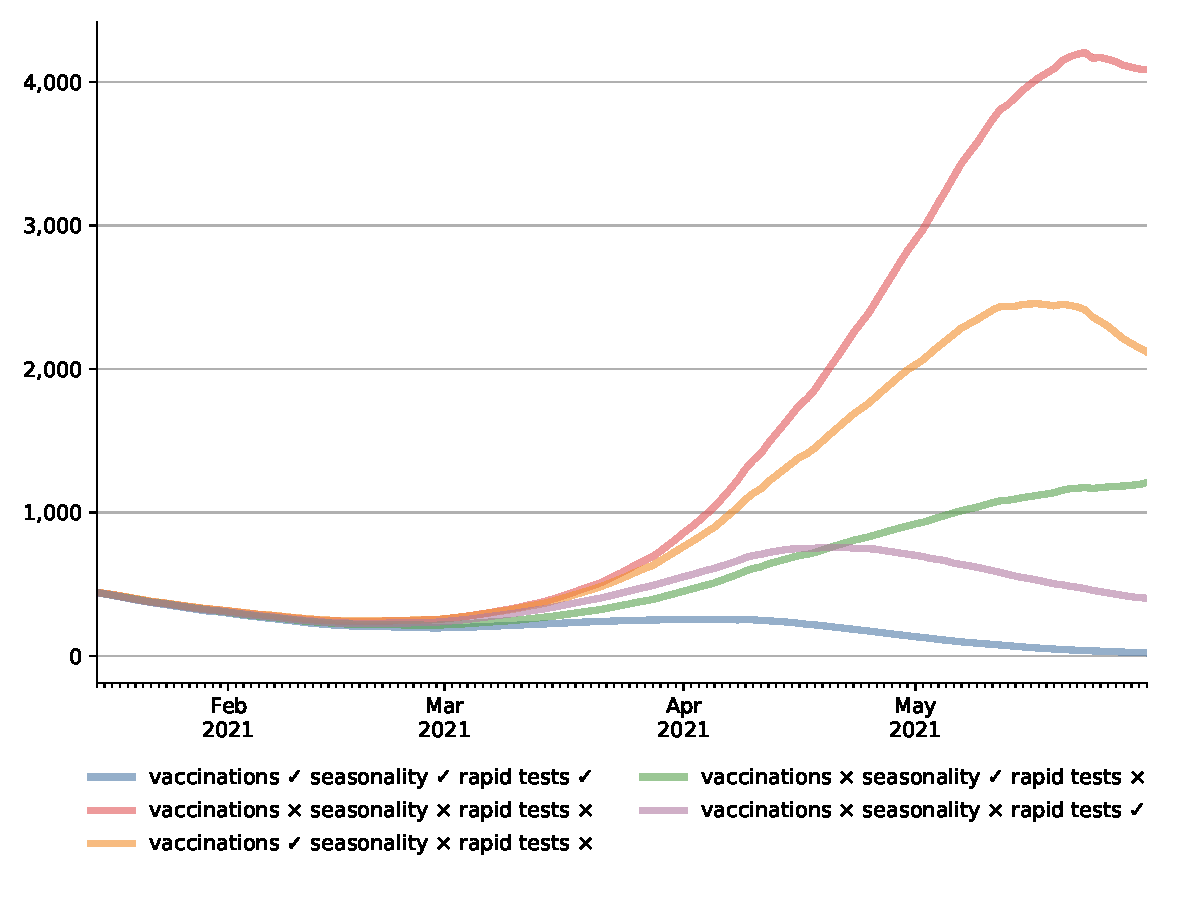
\includegraphics[width=\textwidth]{../figures/results/figures/scenario_comparisons/effect_of_channels_on_pessimistic_scenario/full_newly_infected}
        \caption{{\small Total cases: 2021 scenarios}}
        \label{fig:2021_scenarios_newly_infected}
    \end{subfigure}

    \begin{subfigure}[b]{0.475\textwidth}
        \centering
        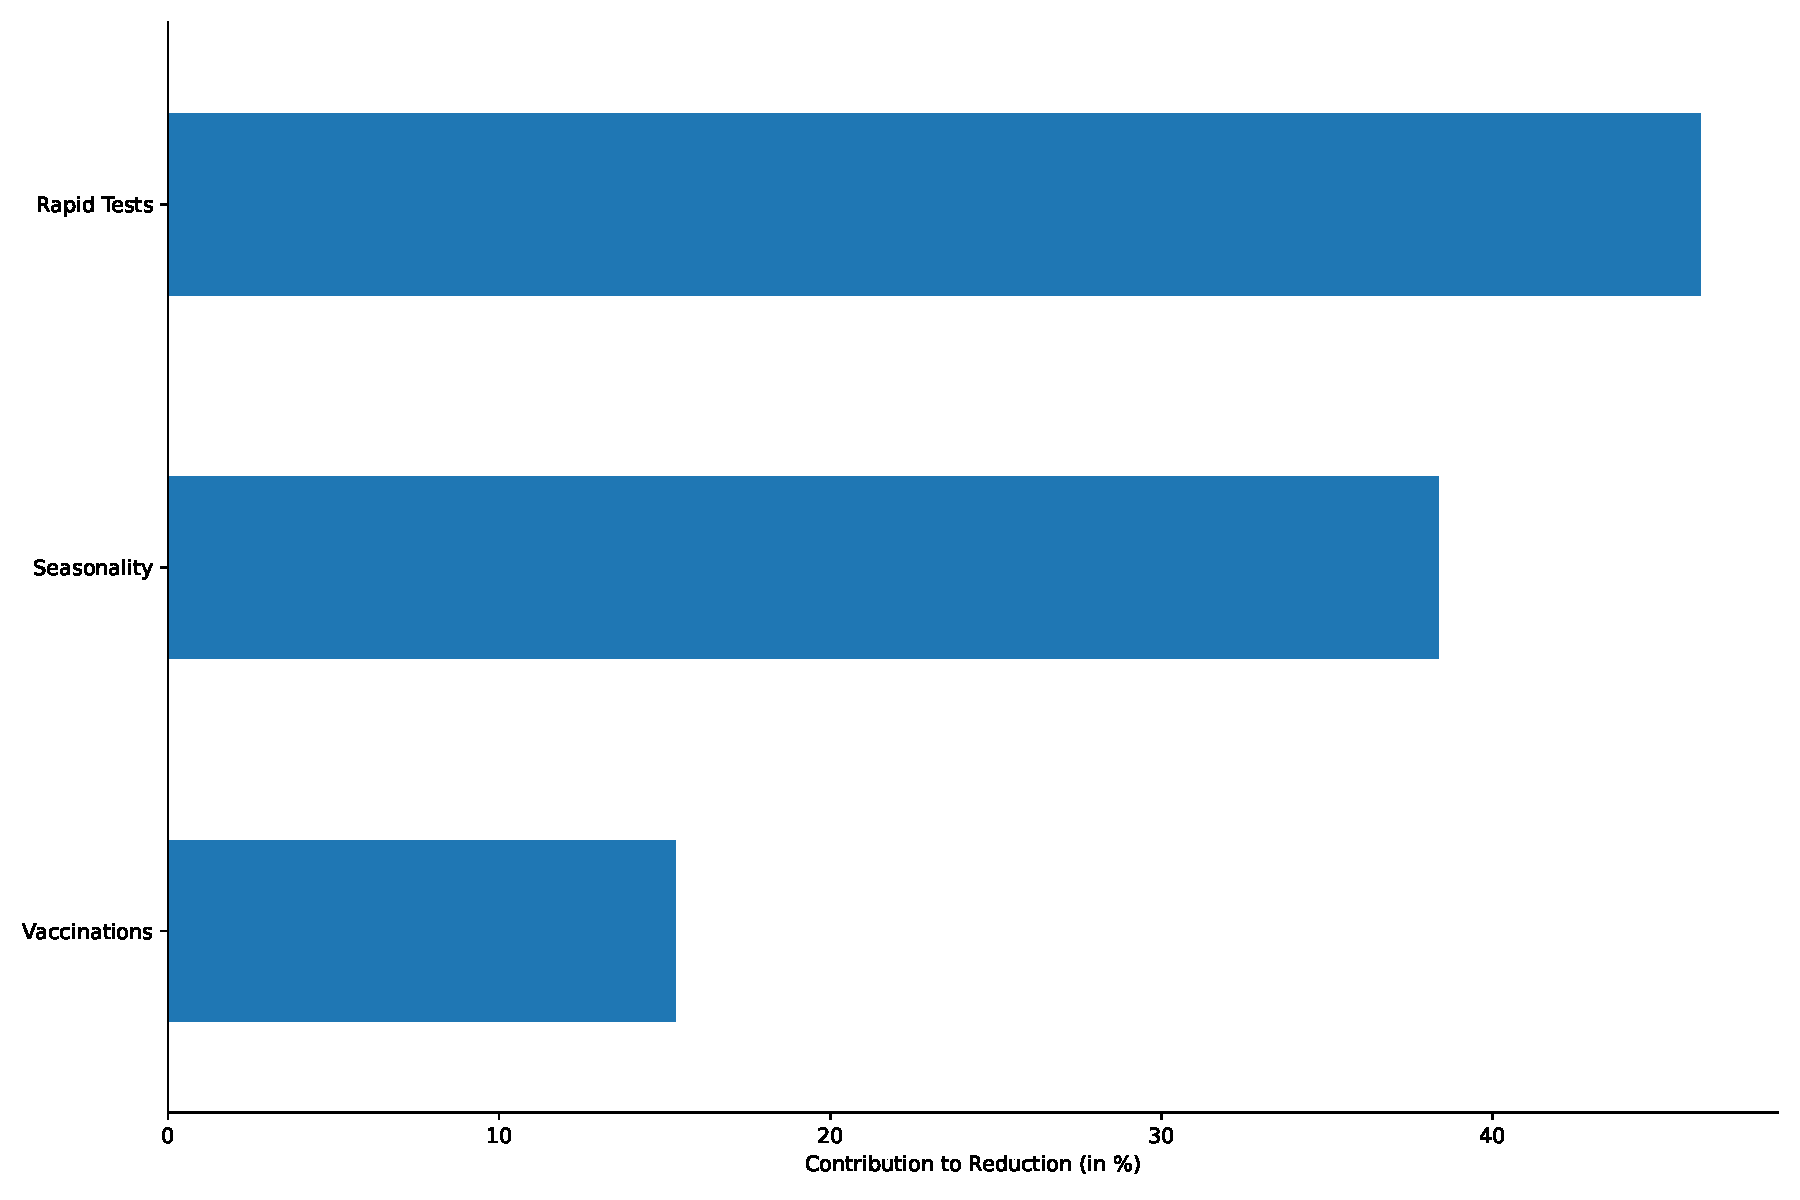
\includegraphics[width=\textwidth]{../figures/full_decomposition}

        \vskip2ex

        \caption{Decomposition of effects for
        Figure~\ref{fig:2021_scenarios_newly_infected}.}
        \label{fig:2021_scenarios_decomposition}
    \end{subfigure}
    \hfill
    \begin{subfigure}[b]{0.475\textwidth}
        \centering

        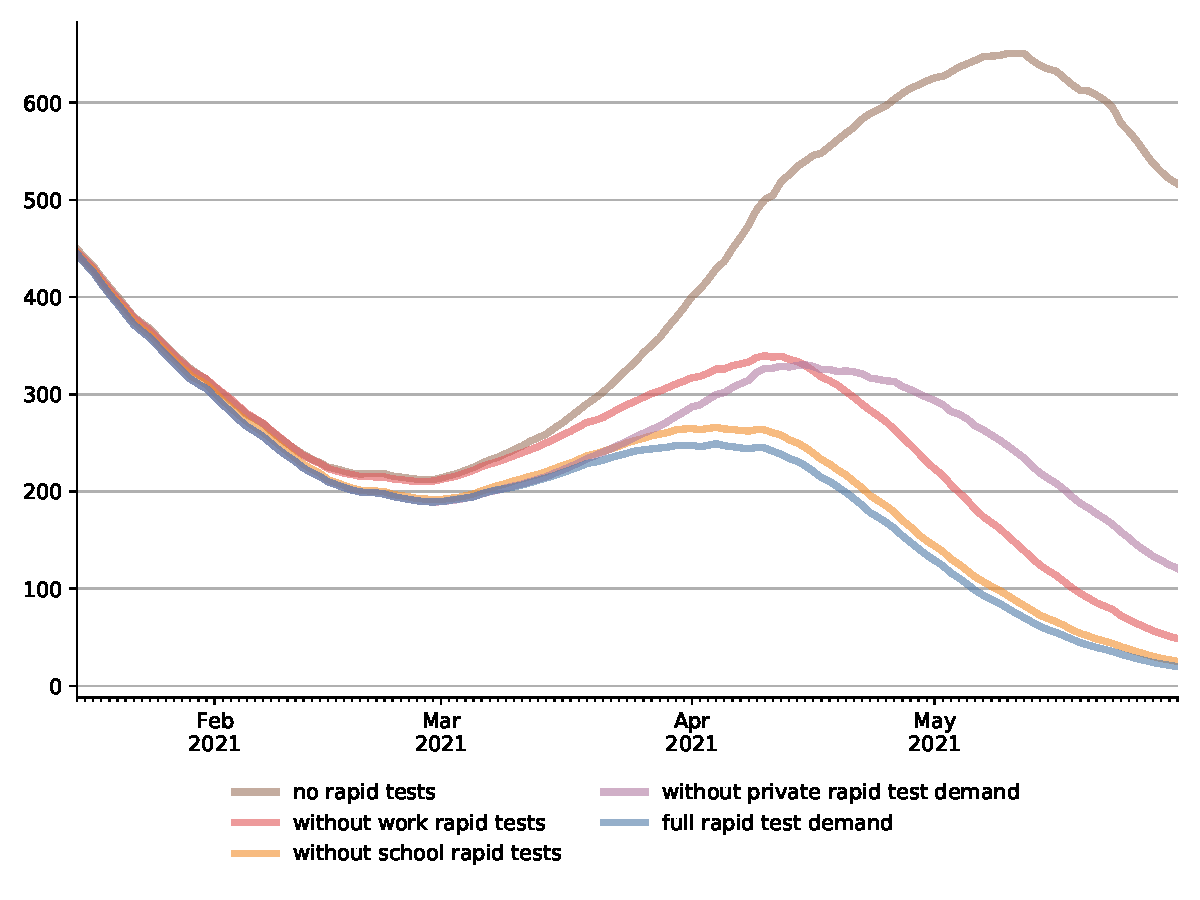
\includegraphics[width=\textwidth]{../figures/results/figures/scenario_comparisons/effect_of_rapid_tests/full_newly_infected}
        \caption{{\small Effects of different types of testing}}
        \label{fig:2021_scenarios_decomposition_tests}
    \end{subfigure}

    \caption{The effect of different interventions on recorded and actual infections}
    \label{fig:2021_scenarios_broad}

    \floatfoot{\noindent Note: All aggregates; See S.XXX for statistics by age group and
    by geographical region.

    The decomposition is based on Shapley values where the individual contribution of a
    channel is its average contribution over different sizes of coalitions (combinations
    with other channels). The individual contribution to a coalition is the difference
    between the effect size of the coalition with the particular channel and without.}
\end{figure}

Until mid-March, there is no visible difference between the different scenarios.
Seasonality hardly changes, and only few vaccinations or rapid tests were administered.
Even thereafter, the effect of the vaccination campaign is surprisingly small at first
sight. Whether considering recorded or total infections, the final level is always the
highest in case the vaccination campaign had been running in isolation (red lines). The
Shapley value decomposition shows that vaccinations contribute about
15\%\comment[id=HM]{check!} to the cumulative difference between scenarios. Reasons for
this are the slow start---it took until 24~March until 10\% of the population had
received their first vaccination, the 20\% mark was reached on April 19th ---and the
focus on older individuals. These groups contribute less to the spread of the disease
than others due to a lower number of contacts, see~\ref{fig:assortativity}. It is
important to note that the initial focus of the campaign was to prevent deaths and
severe disease; the case fatality was rate considerably lower during the third wave when
compared to the second (4.4\% between October and February and 1.4\% between March and
June). It is important to note that by the end of our study period, when first-dose
vaccination rates reached around 40\% of the population, the numbers of new cases would
have started to decline.

Seasonality has a large effect in slowing the spread of SARS-CoV-2. By May 31, both
observed and recorded cases would be reduced by a factor of four if only seasonality
mattered. However, in this period, cases would have kept on rising throughout, just at a
much lower pace. Nevertheless, we estimate it to be a quantitatively important factor
determining the evolution of the pandemic, explaining most of the early changes and
almost 40\% of the cumulative difference by the end of May.

The largest effect---almost one half when considering the decompositions---comes from
rapid testing. Here, it is crucial to differentiate between recorded cases and actual
cases. Additional testing means that infections become known which would otherwise
remain undetected. Figure~\ref{fig:2021_scenarios_recorded} shows that this means that
until late April, recorded cases are higher than in the scenario where none of the three
mechanisms is turned on. Compared to the scenario with vaccinations only, this point is
reached only around mid May and it would be June for the comparison with the
seasonality-only scenario. The effect on total cases, however, kicks in immediately and
strongly. Despite the fact that only a small fraction of the population performed weekly
rapid tests in March (X\%\comment[id=HM]{Put in}), the rise in new infections would be
limited by XXX\% relative to the scenario without vaccinations, tests, or seasonality.

Tests 



\clearpage

Two particularly important areas:
\begin{itemize}
    \item Schooling: large costs to pupils, ... social inequalities
    \item Work: Q2 / 2020 saw the largest drop in GDP in a long time; 
\end{itemize}

Results
\begin{itemize}
    \item Advantage of testing in both cases: Recurrent. Small cost relative to other
    stuff. Certain publicness.
    \item Mandatory tests: Screening effect: ...
\end{itemize}


\begin{figure}[!tp]
    \centering

    \begin{subfigure}[b]{0.475\textwidth}
        \centering
        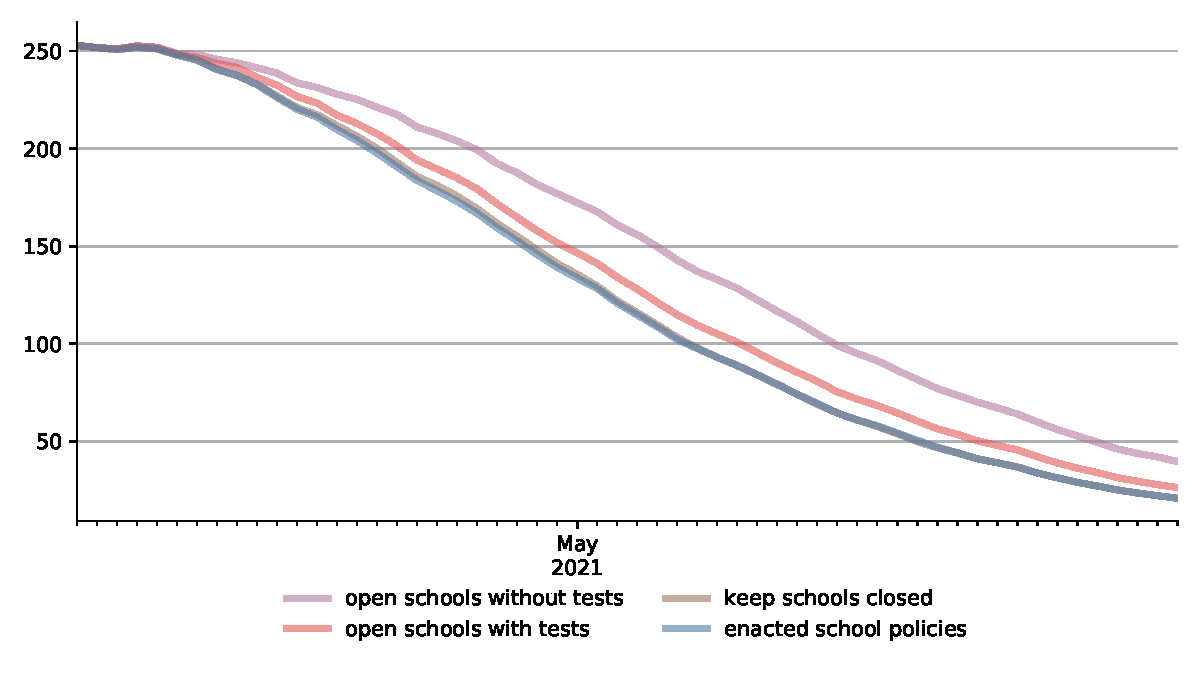
\includegraphics[width=0.9 \textwidth]{../figures/results/figures/scenario_comparisons/school_scenarios/full_newly_infected}
        \caption{{\small Effects of different schooling scenarios after Easter}}
        \label{fig:schooling_scenarios_easter}
    \end{subfigure}
    \hfill
    \begin{subfigure}[b]{0.475\textwidth}
        \centering
        % \includegraphics[width=0.9
        % \textwidth]{../figures/results/figures/scenario_comparisons/}
        \caption{{\small Effects of different work scenarios after Easter}}
        \label{fig:to_be_determined}
    \end{subfigure}
    \vskip3ex

    \caption{Effects of different scenarios for schooling and working from home}
    \label{fig:interventions_school}

    \floatfoot{\noindent Note: All aggregates; See S.XXX for statistics by age group and
        by geographical region.}

\end{figure}




\paragraph{Points to mention}
\begin{itemize}
    \item If anything too optimistic regarding vaccinations
    \item Social structure / conditional block testing in families important (?)
    \item Trump-effect: More testing = more cases true for how long?
\end{itemize}

% Technical terms should be defined. 

% Symbols, abbreviations, and acronyms should be defined the first time they are used. 

% All tables and figures should be cited in numerical order.

% All data must be shown either in the main text or in the Supplementary Materials or
% must be available in an established database with accession details provided in the
% acknowledgements section.

% References to unpublished materials are not allowed to substantiate significant
% conclusions of the paper.


\section{Supplementary Material}

\begin{enumerate}
    \item Model
    \item Data
    \item Identification and Estimation
\end{enumerate}